\chapter*{Ejercicio5}
\section*{5. Disenar un circuito secuencial flip-flop SR, pero utilizando circuitos NAND y
verificar que el resultado es el mismo que con puertas NOR.}

\begin{enumerate}
    \item 
Circuito Flip-Flop SR usando compuertas NAND:
\end{enumerate}

\begin{center}
    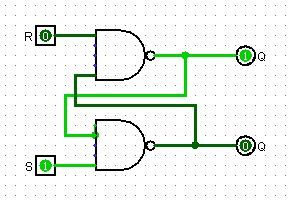
\includegraphics[width=1\textwidth]{recursos/Ejercicio5.png}
\end{center}


